\section{Module Characterization and Benchmarking}

The mechanical design and control strategy were validated by subjecting the custom actuator module to an
experimental characterization mirroring the one applied to to the commercial units in Section
\ref{sec:limitations} The tests were conducted using the integrated AS5600 magnetic sensor for feedback,
with the module powered at a nominal voltage of $6.7\,\text{V}$. The $\text{I}^2\text{C}$ bus was used to
transmit the target position directly as a 12-bit digital setpoint, bypassing the resolution limits of
standard PWM signaling.


\subsection{Static Analysis: Linearity and Hysteresis}

The first validation step focused on the static input-output relationship. A slow triangular ramp reference
($100\,ms$ per sensor LSB) spanning the full range in both Forward and Backward directions was administered
to the module. Figure \ref{fig:custom_linearity} illustrates the experimental results.

Compared to the commercial servo baseline (refer to Figure \ref{fig:servo_deficiencies}), the custom module
demonstrates significant visible improvements:

\begin{itemize}
    \item \textbf{Linearity:} The response closely follows the ideal characteristic $y=x$. The distortion,
        typical of the potentiometer-based commercial unit, is effectively eliminated.
    \item \textbf{Hysteresis Suppression:} The forward and backward paths are virtually indistinguishable at
        full scale. The removal of the mechanical potentiometer in favor of the non-contact magnetic sensor
        drastically reduces mechanical backlash, ensuring high repeatability regardless of the direction of
        approach.
    \item \textbf{Range Extension:} The operating range is no longer constrained by the physical limits of
        the potentiometer, granting access to the full $360^\circ$ of rotation. This continuous capability
        necessitates software phase unwrapping to ensure seamless transitions across the zero-crossing point.
\end{itemize}

\begin{figure}[htbp]
    \centering
    \begin{subfigure}[c]{0.48\textwidth}
        \centering
        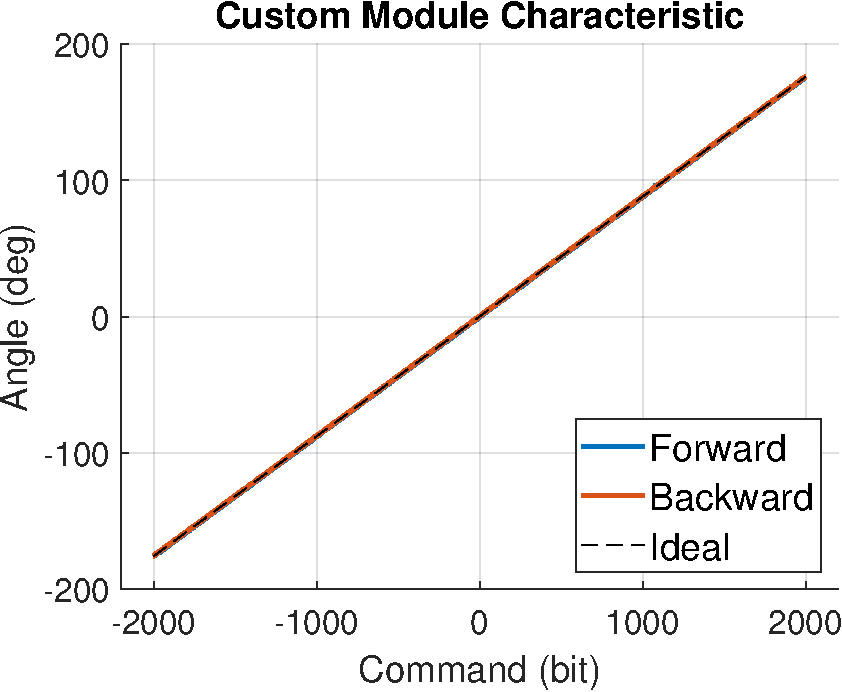
\includegraphics[width=\textwidth]{images/custom_linearity.pdf}
        \caption{Full-scale linearity analysis.}
        \label{fig:custom_linearity_full}
    \end{subfigure}
    \hfill
    \begin{subfigure}[c]{0.48\textwidth}
        \centering
        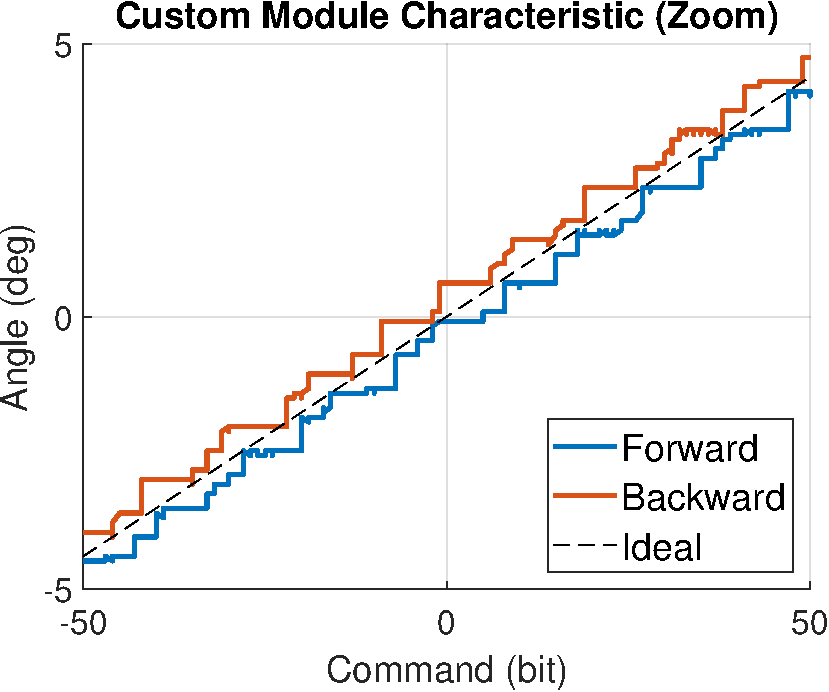
\includegraphics[width=\textwidth]{images/custom_linearity_zoom.pdf}
        \caption{Zoomed view showing micro-linearity.}
        \label{fig:custom_linearity_zoom}
    \end{subfigure}
    \caption{Input-Output Characteristic of the Custom Actuator.}
    \label{fig:custom_linearity}
\end{figure}


\subsection{Step Response Analysis: Sensitivity and Settling}

The module was then subjected to a series of step commands (square waves) of varying amplitudes: Micro-step
($1^\circ$), Mid-range ($15^\circ$), and Full-scale ($90^\circ$).

The results, presented in Figure \ref{fig:step_responses} and \ref{fig:step_error}, highlight two key behaviors:

\begin{itemize}
    \item \textbf{Resolution and Sensitivity ($1^\circ$):} Unlike the commercial unit, which exhibited a
        significant deadband preventing fine adjustments, the custom module responds reliably to micro-step
        commands as small as $1^\circ$ ($\approx 11$ LSB). Note that the visible jitter at this stage is sensor
        noise.
    \item \textbf{Transient Response ($15^\circ, 90^\circ$):} For larger transitions, the motor reaches the
        target setpoint rapidly. While a slight overshoot is visible, the system settles quickly without
        entering a limit cycle (hunting), validating the effectiveness of the Switching PID control algorithm.
\end{itemize}

\begin{figure}[htbp]
\centering
    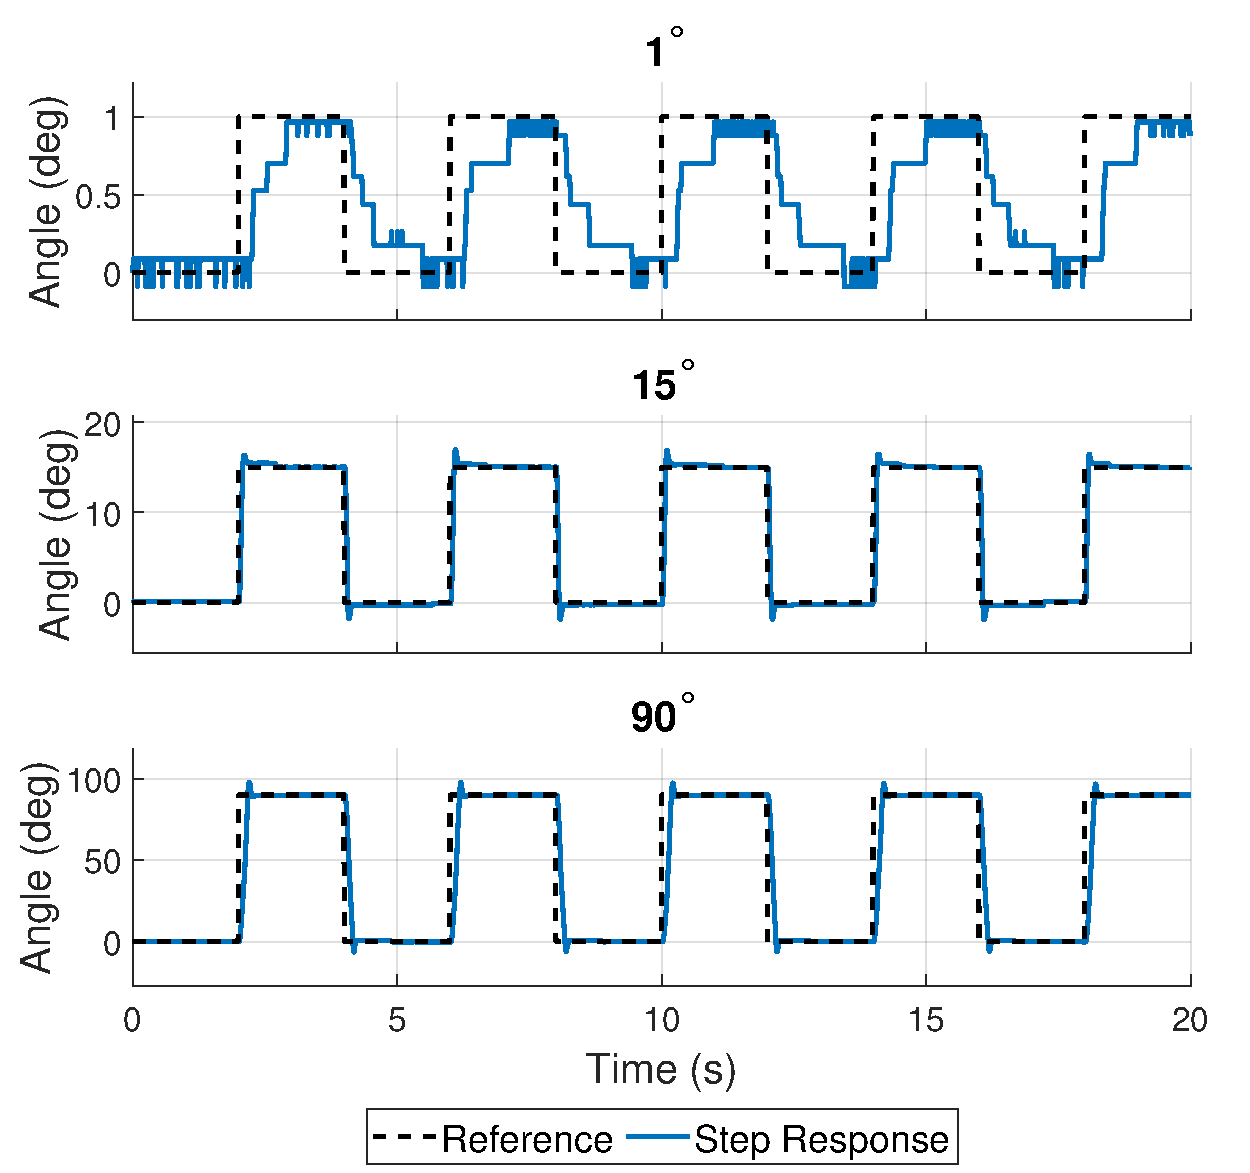
\includegraphics[width=0.98\textwidth]{images/custom_step_response_multi.pdf}
    \caption{Trajectory Tracking}
    \label{fig:step_responses}
\end{figure}

\begin{figure}[htbp]
    \centering
    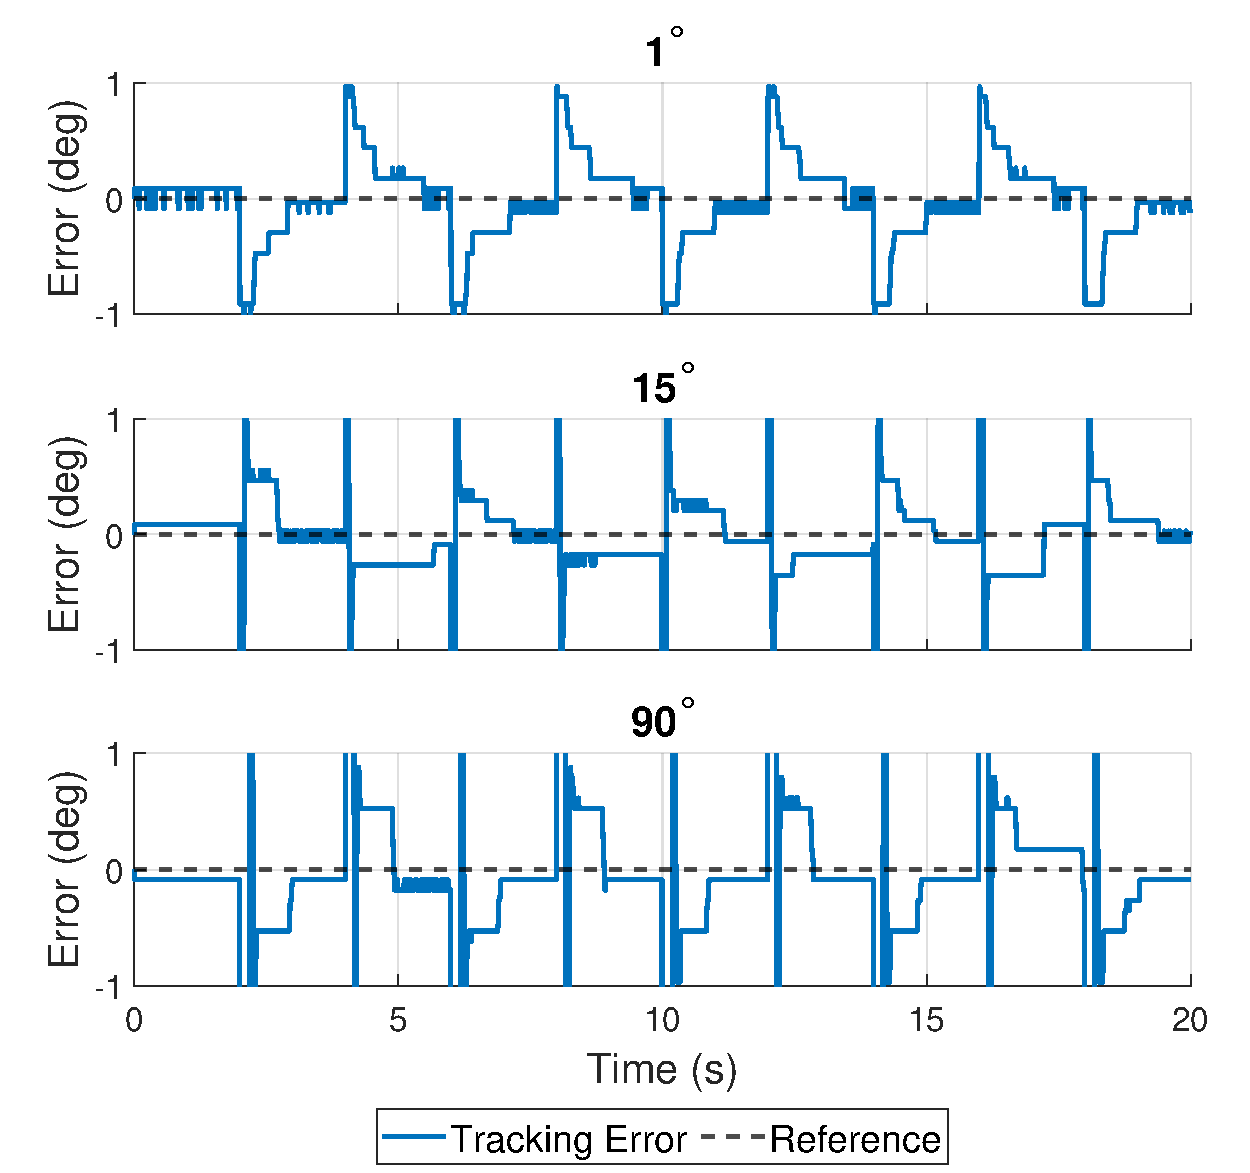
\includegraphics[width=0.98\textwidth]{images/custom_step_error_multi.pdf}
    \caption{Tracking Errors}
    \label{fig:step_error}
\end{figure}


\subsection{Results Summary}

The experimental results confirm that the custom actuator meets the strict requirements of the limb
application. The redesign has yielded a substantial increase in precision, accuracy, and controllability.
The transition to a digital interface ensures scalability and flexibility, while the mechanical form factor
remains compatible with the original design.

To quantify these improvements, a direct benchmark comparison was performed against the two commercial units
characterized in Section \ref{sec:limitations}. Figure \ref{fig:benchmark} illustrates the performance metrics
regarding positioning accuracy and mechanical play.

For the sake of brevity, the mathematical definitions of the metrics used in this analysis (RMSE, Absolute
Error, Hysteresis) are detailed in Appendix \ref{app:metrics}.

\begin{figure}[htbp]
    \centering
    
\includegraphics[width=0.96\textwidth]{images/final_benchmark.pdf}
    \caption{Performance Benchmark Results.}
    \label{fig:benchmark}
\end{figure}

The data reveals a dramatic enhancement in performance:

\begin{itemize}
    \item \textbf{Accuracy:} The Root Mean Square Error (RMSE), which serves as a reliable indicator of
        global linearity and tracking fidelity, dropped from an average of $\approx 14^{\circ}$ in the
        commercial units to just $\mathbf{0.37^{\circ}}$ in the custom prototype. This result comfortably
        satisfies the design requirement of $<\pm 0.5^{\circ}$ set in Section \ref{sec:hardware}.
    \item \textbf{Peak Error:} The Maximum Absolute Error was reduced from extreme values
        ($\approx 29^{\circ}$ for Unit A) to a manageable $\mathbf{1.49^{\circ}}$, effectively eliminating
        the macroscopic non-linearities observed in the analog potentiometers.
    \item \textbf{Hysteresis:} The stick-slip and backlash effects were significantly mitigated. The average
        hysteresis was reduced from $\approx 5^{\circ}$ to $\mathbf{0.65^{\circ}}$, validating the
        effectiveness of the Switching PID strategy in compensating for static friction.
\end{itemize}

Finally, a cost analysis (Appendix \ref{app:bom}) indicates that these performance gains were achieved within
a very limited budget, proving the viability of the proposed custom solution over expensive high-end commercial
alternatives. Further hardware and software improvements can be implemented in the next revision and are left
as future work.